%%%%%%%%%%%%%%%%%%%%%%%%%%%%%%%%%%%%%%%%%%%%%%%%%%%%%%%%%%%%%%%%%%%%%%%%
%                                                                      %
%     File: Thesis_Conclusions.tex                                     %
%     Tex Master: Thesis.tex                                           %
%                                                                      %
%     Author: João C. Godinho                                          %
%     Last modified : May 2018                                         %
%                                                                      %
%%%%%%%%%%%%%%%%%%%%%%%%%%%%%%%%%%%%%%%%%%%%%%%%%%%%%%%%%%%%%%%%%%%%%%%%

\chapter{Conclusions}
\label{chapter:conclusions}

In this work we analyzed how \gls{ml} techniques fit into the scope of malware detection and how could the chosen dataset influence the results of the classifier.
We collected, analyzed, trained and validated multiple datasets to better understand how \textit{laboratory conditions} vary from \textit{real-world conditions}.
Doing so provided us with \gls{auroc} results varying from as high as 98\% to as low as 67\%.

Given the non-existence of a common agreement on how to label samples in a real world dataset, we have proposed three different metrics $\Mrealv$, $\Mloosev$ and $\Mstrictv$ for labeling these samples, and presented three different scenarios $\mathcal{S}_{strict}$, $\mathcal{S}_{loose}$ and $\mathcal{S}_{real}$, ranging from a more simulated scenario, to more realistic ones.

We have analyzed the different scenarios mainly on two kind of conditions: the \textit{laboratory conditions} where the standard cross-validation methodology was applied discarding the importance of \emph{time} in malware detection, and temporal consistent techniques where we have trained and validated the model in a temporal consistent manner.
We have shown that for a modest compromise in accuracy temporal consistent methodologies are adequate to classify malware samples.

We have also concluded that we can reduce the size of the training dataset to avoid the need of training with all ever seen samples, and argue on how much it can be reduced without compromising optimal results.

Having solid knowledge on the effects of temporal consistency in the task of malware detection, we improved our base model for better results.
This was done by using a multi layer approach to provide the ability to extract information regarding malware classes, and by adding more features to the model.
These improvements boosted our results between 7\% and 20\%, while still guaranteeing temporal consistency.

To show our confidence in the obtained results, we provided two practical applications of our developed model, still under development, but with hopes of being implemented in a production environment soon.

We believe that the pertinent question of how much should we seek for great results on \gls{ml} techniques applied to malware detection is worth to be further discussed, bearing in mind that it leads to classifiers that would not perform better over realistic conditions.

The task we set ourselves to achieve was not without its difficulties, but all in all, we believe our work shows that the path to malware detection via machine learning is feasible, not only theoretically, as related work as shown, but also with practical implications.


% TODO mudar pratical para aqui


\section{Practical Applications}
\label{section:practical_applications}

We take this section to briefly describe how we took the previously defined model to the real world, providing practical implementations for it.
The following work is still on-going as part of a scholarship provided by INOV - Inesc Inovação, as such the end products are still being developed and test.

%%%%%%%%%%%%%%%%%%%%%%%%%%%%%%%%%%%%%%%%%%%%%%%%%%%%%%%%%%%%%%%%%%%%%%%%
\subsection{Malware Detection Service}
\label{section:malware_service}

Our first practical application for the obtained model comes as a malware detection service.
The idea is to take advantage of Cuckoo~\cite{tool:cuckoo} to implement a web service identical to Malwr~\cite{tool:malwr}, but also adding the malware detection by applying our model.

To implement this service, we developed a simple web application that receives files from users and then sends them to a Cuckoo instance running on a server.
We created a custom signature for Cuckoo that takes the analysis results and converts it into features suitable for our model, which is then used to classify the sample.
The output of the model is then appended as a signature to the final report.
After analysis our web application extracts basic information regarding the file, as well as the output of the classifier.

We implemented our web application using Django~\cite{tool:django}.
The implemented application provides a simple upload form for users to submit their own files.
Upon submission, Django sends the sample to a Cuckoo instance running locally.
While Cuckoo is analyzing the sample, users are redirected to the report page, which shows the current state of analysis.
Upon finishing analysis, the page changes to yield the classifier results.

Figure \ref{fig:malware_detetor} shows the service being tested with a \texttt{petya}\footnote{Symantec - Petya Ransomware, October 27, 2017 [https://www.symantec.com/blogs/threat-intelligence/petya-ransomware-wiper]} sample, using early versions of our $\LR$ model.

\begin{figure}[!h]
	\centering
	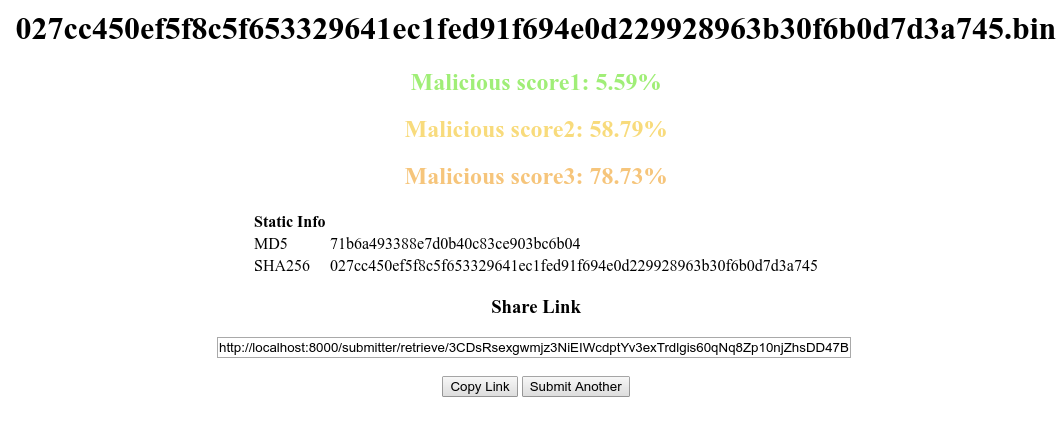
\includegraphics[width=0.8\textwidth]{Figures/malware_detector.png}
	\caption{Malware Detector in early stages.}
	\label{fig:malware_detetor}
\end{figure}

We are currently testing and optimizing the service, as it is not currently using our latest and best model $\mathcal{E}$.

%%%%%%%%%%%%%%%%%%%%%%%%%%%%%%%%%%%%%%%%%%%%%%%%%%%%%%%%%%%%%%%%%%%%%%%%
\subsection{Email Attachment Scanner}
\label{section:email_scanner}

Our second practical application uses the previous service, but in an automated way, to scan email attachments arriving and departing INOV's mail server.
The idea is to insert the malware detector in the mail server pipeline as a scanner.

INOV's mail server uses MailScanner~\cite{tool:mailscanner} to filter and scan emails.
In Figure \ref{fig:mailscanner} we provide a diagram on the MailScanner pipeline.

Our implementation works by creating a custom \textit{Virus Scanner}, which takes email attachments and sends them to the previous described malware detection service.
Upon receiving the results, our custom scanner modifies the mail object to include the classification results.

Further down in the \textit{Message Processing} step, we added a custom step to modify an unused \texttt{Header} in the email to include the classification results.

Currently we are in the process of moving the developed code into the mail server to start obtaining real world results.

\begin{figure}[!h]
	\centering
	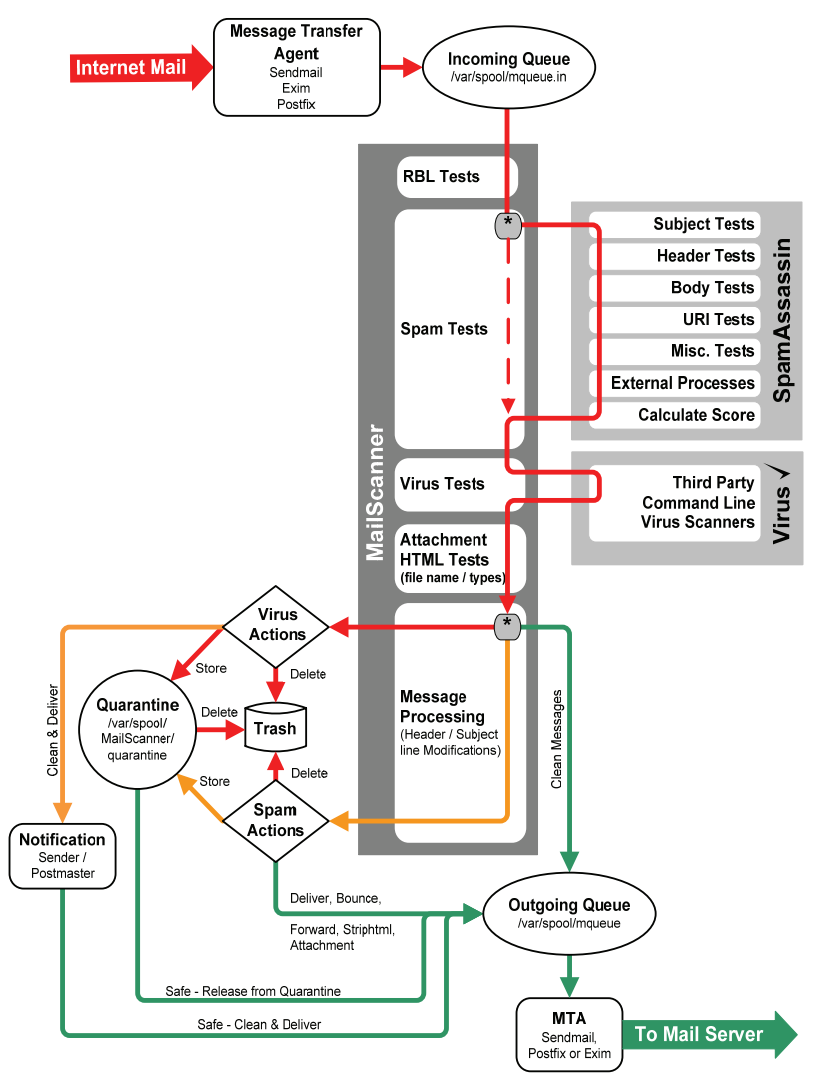
\includegraphics[width=0.8\textwidth]{Figures/mailscanner.png}
	\caption{MailScanner process diagram.}
	\label{fig:mailscanner}
\end{figure}


% ----------------------------------------------------------------------
\section{Achievements}
\label{section:achievements}

In summary, in this work we achieved the following results:

\begin{itemize}
	\item We provided means to achieve metrics as to facilitate the malware labeling task.
	\item We developed methodologies that test real-world scenarios which take into account time consistency, rather than laboratory created scenarios.
	\item We provided a simple model to detect malware and investigated how it behaves under different methodologies.
	\item We improved the previous model with a two layer approach and more dynamic features to boost the results in all of our tested methodologies.
	\item We started developing practical applications of our model, to be inserted in real world scenarios.
\end{itemize}

% ----------------------------------------------------------------------
\section{Future Work}
\label{section:future}

As future work, the developed model could be improved by adding more features, and by doing more in depth research regarding the impacts of each feature.
Other models could be tested, as well as used in conjunction with our logistic regression, to improve the overall results.
Diverging from a supervised learning methodology to include other types of learning would also bring benefits and possibly achieve a fully automated pipeline to detect malware, with minimal user interaction.
